\documentclass[12pt]{article}

\usepackage{amsmath, mathtools}
\usepackage{amsfonts}
\usepackage{amssymb}
\usepackage{graphicx}
\usepackage{colortbl}
\usepackage{xr}
\usepackage{hyperref}
\usepackage{longtable}
\usepackage{xfrac}
\usepackage{tabularx}
\usepackage{float}
\usepackage{siunitx}
\usepackage{booktabs}
\usepackage{caption}
\usepackage{pdflscape}
\usepackage{afterpage}
\usepackage{caption}
\usepackage{pbox}
\usepackage{makecell}
\usepackage[mathscr]{euscript}
\externaldocument{../VnVPlan/SystVnVPlan/SystVnVPlan}

\DeclareSymbolFont{rsfs}{U}{rsfs}{m}{n}
\DeclareSymbolFontAlphabet{\mathscrsfs}{rsfs}

\usepackage[sort&compress,square,comma,numbers]{natbib}

\DeclareRobustCommand{\citeext}[1]{\citeauthor{#1}~\cite{#1}}

%\usepackage{refcheck}

\hypersetup{
    bookmarks=true,         % show bookmarks bar?
      colorlinks=true,       % false: boxed links; true: colored links
    linkcolor=red,          % color of internal links (change box color with linkbordercolor)
    citecolor=blue,        % color of links to bibliography
    filecolor=magenta,      % color of file links
    urlcolor=cyan           % color of external links
}

%% Comments

\usepackage{color}

\newif\ifcomments\commentstrue

\ifcomments
\newcommand{\authornote}[3]{\textcolor{#1}{[#3 ---#2]}}
\newcommand{\todo}[1]{\textcolor{red}{[TODO: #1]}}
\else
\newcommand{\authornote}[3]{}
\newcommand{\todo}[1]{}
\fi

\newcommand{\wss}[1]{\authornote{blue}{SS}{#1}} 
\newcommand{\plt}[1]{\authornote{magenta}{TPLT}{#1}} %For explanation of the template
\newcommand{\an}[1]{\authornote{cyan}{Author}{#1}}

%% Common Parts

\newcommand{\progname}{ProgName} % PUT YOUR PROGRAM NAME HERE %Every program
                                % should have a name



% For easy change of table widths
\newcommand{\colZwidth}{1.0\textwidth}
\newcommand{\colAwidth}{0.13\textwidth}
\newcommand{\colBwidth}{0.82\textwidth}
\newcommand{\colCwidth}{0.1\textwidth}
\newcommand{\colDwidth}{0.05\textwidth}
\newcommand{\colEwidth}{0.8\textwidth}
\newcommand{\colFwidth}{0.17\textwidth}
\newcommand{\colGwidth}{0.5\textwidth}
\newcommand{\colHwidth}{0.28\textwidth}

% Used so that cross-references have a meaningful prefix
\newcounter{defnum} %Definition Number
\newcommand{\dthedefnum}{GD\thedefnum}
\newcommand{\dref}[1]{GD\ref{#1}}
\newcounter{datadefnum} %Datadefinition Number
\newcounter{goalnum} %Datadefinition Number
\newcommand{\ddthedatadefnum}{DD\thedatadefnum}
\newcommand{\ddref}[1]{DD\ref{#1}}
\newcounter{theorynum} %Theory Number
\newcommand{\tthetheorynum}{T\thetheorynum}
\newcommand{\tref}[1]{T\ref{#1}}
\newcounter{tablenum} %Table Number
\newcommand{\tbthetablenum}{T\thetablenum}
\newcommand{\tbref}[1]{TB\ref{#1}}
\newcounter{assumpnum} %Assumption Number
\newcommand{\atheassumpnum}{P\theassumpnum}
\newcommand{\aref}[1]{A\ref{#1}}
%\newcounter{goalnum} %Goal Number
\newcommand{\gthegoalnum}{P\thegoalnum}
\newcommand{\gsref}[1]{GS\ref{#1}}
\newcounter{instnum} %Instance Number
\newcommand{\itheinstnum}{IM\theinstnum}
\newcommand{\iref}[1]{IM\ref{#1}}
\newcounter{reqnum} %Requirement Number
\newcommand{\rthereqnum}{P\thereqnum}
\newcommand{\rref}[1]{R\ref{#1}}
\newcounter{lcnum} %Likely change number
\newcommand{\lthelcnum}{LC\thelcnum}
\newcommand{\lcref}[1]{LC\ref{#1}}

\newcommand{\famname}{Lattice Boltzmann Solvers} % PUT YOUR PROGRAM NAME HERE

\usepackage{fullpage}

\begin{document}

\title{\famname} 
\author{Peter Michalski}
\date{\today}

\maketitle

~\newpage

\pagenumbering{roman}

\section{Revision History} \label{CAREVHISTORY}

\begin{tabularx}{\textwidth}{p{3cm}p{2cm}X}
\toprule {\bf Date} & {\bf Version} & {\bf Notes}\\
\midrule
Oct. 7,2019 & 1.0 & Initial Document\\
Oct. 20,2019 & 1.1 & First Issues Fixed + 10.4 Added\\
Nov. 9,2019 & 2.0 & Iteration One Issues Fixed\\
\bottomrule
\end{tabularx}

~\newpage
	
\section{Reference Material}

This section records information for easy reference.

\subsection{Table of Units}

Throughout this document SI (Syst\`{e}me International d'Unit\'{e}s) is employed
as the unit system.  In addition to the basic units, several derived units are
used as described below.  For each unit, the symbol is given followed by a
description of the unit and the SI name.
~\newline

\renewcommand{\arraystretch}{1.2}
%\begin{table}[ht]
  \noindent \begin{tabular}{l l l} 
    \toprule		
    \textbf{symbol} & \textbf{unit} & \textbf{SI}\\
    \midrule 
    $cm$ & length & centimetre\\
    $g$ & mass & gram \\
    $kg$ & mass	& kilogram\\
    $m$ & length & metre\\
    $N$ & force & newton\\
    $Pa$ & pressure & pascal\\
    $s$ & time & second\\
    \bottomrule
  \end{tabular}
  %	\caption{Provide a caption}
%\end{table}

\subsection{Table of Symbols}

The table that follows summarizes the symbols used in this document along with
their units.  The choice of symbols was made to be consistent with Lattice Boltzmann Method literature and with existing documentation for Lattice Boltzmann Methods. The symbols are listed in alphabetical order. Boldface represents vector units.

\renewcommand{\arraystretch}{1.2}
%\noindent \begin{tabularx}{1.0\textwidth}{l l X}
\noindent \begin{longtable*}{l l p{12cm}} \toprule
\textbf{symbol} & \textbf{unit} & \textbf{description}\\
\midrule 
$\mathrm{a}$ & $\frac{m}{s^2}$ & acceleration rate
\\
$A$ & $m^2$ & cross-sectional area
\\
$\textbf{c}_\textbf{i}$ & N/A & unit vector along the lattice streaming direction
\\
$c_s$ & $\frac{m}{s}$ & speed of sound
\\
$\mathrm{D}$ & N/A & signifies the dimension component of lattice model
\\
$\mathscr{D}$ & N/A & denotes DD in Table \ref{table:tracemodels}
\\
$\mathrm{e}$ & $\frac{m}{s}$ & velocity
\\
$\eta$ & $\si{\pascal}\cdot\si{\second}$ & viscosity %\wss{The units are not shown correctly.  (The font is incorrect, and the units themselves should be pascal seconds (Pa times s).I suggest using the si package, as in the SRS.tex example.}
\\ 
$f$ & N/A & distribution function
\\
$f^{eq}$ & N/A & equilibrium distribution function
\\
$F$ & $N$ & force
\\
$\gamma$ & $\frac{1}{s}$ & velocity gradient
\\
$i$ & N/A & velocity direction (linkages of lattice model)
\\
$l$ & $m$ & characteristic length of the system
\\
$\nabla$ & N/A & gradient
\\
$\mathbb{N}$ & N/A & natural numbers
\\
$\Omega$ & N/A & collision operator
\\
$\mathrm{Q}$ & N/A & signifies number of velocity directions of lattice model
\\
$\rho$ & $\frac{g}{cm^3}$ & fluid density
\\
$\mathbb{R}$ & N/A & real numbers
\\
$Re$ & N/A & Reynolds number
\\
$t$ & $s$ & time
\\
$\tau$ & N/A & relaxation rate
\\
\textbf{u} & $\frac{m}{s}$ & macroscopic velocity of fluid vector
\\
$w$ & N/A & weight coefficient (implementation specific)
\\
\textbf{x} & N/A & position vector
\\
$z$ & N/A & position of a fluid
\\
$\zeta$ & N/A & turbulence
\\
$?$ & N/A & unknown value 
\\
\bottomrule
\end{longtable*}

\subsection{Abbreviations and Acronyms}

\renewcommand{\arraystretch}{1.2}
\begin{tabular}{l l} 
  \toprule		
  \textbf{symbol} & \textbf{description}\\
  \midrule
  1D & 1-Dimensional\\ 
  2D & 2-Dimensional\\ 
  3D & 3-Dimensional\\ 
  A & Assumption\\
  AHP & Analytic Hierarchy Process\\
  CA & Commonality Analysis\\
  DD & Data Definition\\
  GS & Goal Statement\\
  LBM & Lattice Boltzmann Methods\\
  LBS & Lattice Boltzmann Solvers\\
  LC & Likely Change\\
  MG & Module Guide\\
  MIS & Module Interface Specification\\
  MPI & Message Passing Interface\\
  MTBF & Mean Time Between Failures\\
  NFR & Non-Functional Requirement\\
  NNF & Non-Newtonian Fluid\\
  OTS & Off The Shelf (LBM Solutions)\\
  PNG & Portable Network Graphics\\
  R & Requirement\\
  T & Theoretical Model\\
  VnV & Verification and Validation\\
  \bottomrule
\end{tabular}\\

\newpage

\tableofcontents

\pagenumbering{arabic}
\newpage
\section{Introduction}

This document provides a Commonality Analysis (CA) for a family of Lattice Boltzmann Solvers (LBS), which provide services based on Lattice Boltzmann Methods (LBM).
LBM are a family of fluid dynamics algorithms for simulating single-phase and multiphase fluid flows, often incorporating additional physical complexities (\citet{chen1998lattice}). They consider the behaviours of a collection of particles as a single unit at the mesoscopic scale. These methods predict the positional probability of a collection of particles moving through a lattice structure. Off the shelf (OTS) Lattice Boltzmann Solvers (LBS) allow for a range of fluid and physical model input parameters, computational parameters, and output parameters as outlined in Section \ref{OTSsolutions}.
The following subsections of this introduction will outline the purpose of this document, a general scope of the family of LBS, the characteristics of the intended reader, and finally an outline of the rest of this document.

\subsection{Purpose of Document}

The purpose of this document is to provide general information on currently available LBS solutions, including their commonalities and variabilities, as well as a baseline understanding of the model and structure of abstract LBM. The information provided here will be used in the development of the design of a solution providing services of a family of LBS.

\subsection{Scope of the Family}
\label{scopeoffamily} 

The family of LBS will model one or more fluids as they pass through a boundary, modeled by a lattice. Fluids with any properties can be modeled, however only those properties that are accepted as inputs by the LBS will affect the model results. The calculation of the LBM distribution function will use 1D, 2D, and 3D computational models, and will output the data into memory and render it on a screen in up to 3D imaging. The output results can also be rendered to a file.\\

\begin{figure}[h!]
\begin{center}
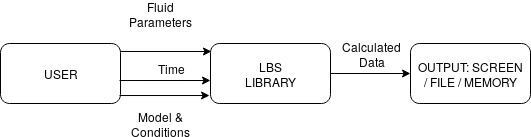
\includegraphics[width=0.8\textwidth]{SystemContext}
\caption{LBS Family Scope}
\label{Fig_SystemContext}
\end{center}
\end{figure}

\subsection{Characteristics of Intended Reader} 

The intended reader of this document should have an undergraduate understanding of software requirements specifications and software design principles. Ideally, they will also have at least an undergraduate Level 3 physics understanding, including of lattice structures and fluid dynamics.

\subsection{Organization of Document}

This document is organized following a template for a CA for scientific computing software proposed by \citet{smith2006systematic}. It follows a standard pattern of presenting a general system description, commonalities, variabilities, and the requirements for a family of LBS. The goal statements of the family of LBS, found in Section \ref{goalstatements}, are refined to the theoretical models in Section \ref{sec_theoretical}. Variabilities within the family are found in Section \ref{variabilities}. Tables of OTS solution commonalities and variabilities are found in Section \ref{OTSsolutions}.

~\newpage

\section{General System Description}

This section identifies the interfaces between the system and its environment,
describes the potential user characteristics, and lists the potential system
constraints.

\subsection{Potential System Contexts}

\begin{itemize}
\item User Responsibilities:
\begin{itemize}
\item The user must provide the system with correctly formatted physical model parameters.
\item The user must select the desired mathematical model for the computation.
\item The user must select the desired format of output for the model.
\end{itemize}
\item \famname{} Responsibilities:
\begin{itemize}
\item Detect data type mismatch, such as a negative number instead of a positive number for a parameter (for example, $A$ cannot accept negative values).
\item Initialize the correct data types and data structures for the model.
\item Perform the calculations to predict the distribution of fluid particles over time.
\item Store the distribution function output data.
\item Store calculated fluid parameters over time.
\item Visually model the results of the distribution function.
\item Store the calculation results in a file and/or in memory.
\item Detect errors during parameter input, model calculation, or model output; store the errors in a file and show the error to the user.
\item Recover from error states, such as those that develop from division by zero or a buffer overflow.
\end{itemize}
\end{itemize}

\subsection{Potential User Characteristics} \label{SecUserCharacteristics}

The end user of \famname{} should ideally have an understanding of undergraduate Level 1 physics and fluid dynamics. The ideal end user characteristics may differ between the members of the family of solvers. For example, a user of HemeLB, an off the shelf LBM solution for simulating blood flow, would ideally have an understanding of phlebology.

~\newpage

\section{Commonalities}

\subsection{Background Overview} \label{Sec_Background}

As LBS model fluid dynamics within a boundary using a predefined lattice structure, the methods rely on a two step calculation process. The first process is streaming, where the particles move along the lattice via links. The second process is collision, where energy and momentum is transferred among particles that collide \cite{bao2011lattice}.
There are many standardized lattice models - individual solvers within the family might only use a subset of them.
The LBM uses the initial parameters of the fluid to find the probability of where along the lattice linkages a group of particles are most likely to travel. It then moves the particles into the next node, and transfers the energy and momentum if a collision occurs. Then the process repeats for the duration of the modeling instance.

~\newpage

\subsection{Terminology and  Definitions}
\label{termdef}

This subsection provides a list of terms that are used in the subsequent
sections and their meaning, with the purpose of reducing ambiguity and making it
easier to correctly understand the requirements:

\begin{itemize}

\item Correctness: The degree to which a system or component is free from faults in its specification, design, and implementation (\citet{IEEEStdGlossarySET1990}).
\item Maintainability: The ease with which a software system or component can be modified to correct faults, improve performance or other attributes, or adapt to a changed environment (\citet{IEEEStdGlossarySET1990}).
\item Performance: The degree to which a system or component accomplishes its designated functions within given constraints, such as speed, accuracy, or memory usage (\citet{IEEEStdGlossarySET1990}).
\item Portability: The ease with which a system or component can e transferred from one hardware or software environment to another (\citet{IEEEStdGlossarySET1990}).
\item Reliability: The ability of a system or component to perform its required functions under stated conditions for a specified period of time (\citet{IEEEStdGlossarySET1990}).
\item Reusability: The degree to which a software module or other work product can be used in more than one computer program or software system (\citet{IEEEStdGlossarySET1990}).
\item Robustness: The degree to which a system or component can function correctly in the presence of invalid inputs or stressful environmental conditions (\citet{IEEEStdGlossarySET1990}).
\item Scalability: The ability of the system to cope with increasing numbers of users without reducing overall QoS that is delivered to any user (\citet{sommerville}).
\item Understandability: The ease of understanding the software system  (\citet{uchida2005experiment}).
\item Usability: The ease with which a user can learn to operate, prepare inputs for, and interpret outputs of a system or component (\citet{IEEEStdGlossarySET1990}).
\item Velocity Directions (Q): The number of links connecting to each lattice node in the chosen model from neighbouring nodes. All nodes in a chosen lattice model will have the same number of links. A single link will connect between two adjacent nodes.
\item D\#Q\# Convention: This signifies the dimension (D) and velocity direction (Q) components of a lattice model. For example, D2Q9 signifies a 2D lattice model with 9 velocity directions out of each node.

\end{itemize}

~\newpage

\subsection{Data Definitions} \label{sec_datadef}

This section collects and defines all the data needed to build the instance models. The dimension of each quantity is also given.  

~\newline

\noindent
\begin{minipage}{\textwidth}
\renewcommand*{\arraystretch}{1.5}
\begin{tabular}{| p{\colAwidth} | p{\colBwidth}|}
\hline
\rowcolor[gray]{0.9}
Number& DD\refstepcounter{datadefnum}\thedatadefnum \label{DD_Velocity}\\
\hline
Label& \bf Velocity\\
\hline
Symbol &$\mathrm{e}$\\
\hline
% \hline
  SI Units & $\frac{m}{s}$\\
  \hline
  Equation& $\mathrm{e} = \frac{d \mathrm{\textbf{x}}}{dt}$\\
  \hline
  Description & 
                 Velocity is the distance that an object moves relative to time. \textbf{x} is the position vector. $t$ is time.
  \\
  \hline
  Sources& \citet{mohamad2011lattice}\\
  \hline
  Ref.\ By & A\ref{A_fluids} DD\ref{DD_VELVIR} IM\ref{lbmim1} \tref{T_ReynoldsNum} \tref{T_CFBTE} \tref{T_BTE} \\
  \hline
\end{tabular}
\end{minipage}\\

~\newline

\noindent
\begin{minipage}{\textwidth}
\renewcommand*{\arraystretch}{1.5}
\begin{tabular}{| p{\colAwidth} | p{\colBwidth}|}
\hline
\rowcolor[gray]{0.9}
Number& DD\refstepcounter{datadefnum}\thedatadefnum \label{DD_Viscosity}\\
\hline
Label& \bf Viscosity\\
\hline
Symbol &$\mathrm{\eta}$\\
\hline
% \hline
  SI Units & $\si{\pascal}\cdot\si{\second}$\\
  \hline
  Equation& $\mathrm{\eta} = \frac{F/A}{\gamma}$\\
  \hline
  Description & 
                Viscosity is the measure of resistance to deformation. $F$ is the applied force ($N$), $A$ is the cross-sectional area ($m^2$), and $\gamma$ is the velocity gradient. 
  \\
  \hline
  Sources& \citet{viscosity}\\
  \hline
  Ref.\ By & A\ref{A_fluids} A\ref{A_fluids} DD\ref{DD_RelaxationRate} \tref{T_ReynoldsNum} \\
  \hline
\end{tabular}
\end{minipage}\\

~\newline

\noindent
\begin{minipage}{\textwidth}
\renewcommand*{\arraystretch}{1.5}
\begin{tabular}{| p{\colAwidth} | p{\colBwidth}|}
\hline
\rowcolor[gray]{0.9}
Number& DD\refstepcounter{datadefnum}\thedatadefnum \label{DD_RelaxationRate}\\
\hline
Label& \bf Relaxation Rate Towards Equilibrium\\
\hline
Symbol &$\tau$\\
\hline
% \hline
  SI Units & N/A\\
  \hline
  Equation&$\tau = \frac{12\mathrm{\eta}\Delta t}{\Delta\mathrm{\textbf{x}}^2} + \frac{1}{2}$\\
  \hline
  Description & 
                The relaxation rate defines how quickly the particles recover to equilibrium state. Adjusting this method in the implementation allows for the simulation of complex physical phenomena, specifically concerning the fluid media. $\mathrm{\eta}$ is the viscosity of the fluid, $t$ is the time interval (s), and \textbf{x} is the position vector.
  \\
  \hline
  Sources& \citet{lbmbolton}\\
  \hline
  Ref.\ By & A\ref{A_fluids} A\ref{A_selectModel} DD\ref{DD_BGK} DD\ref{DD_RELUPD}\\
  \hline
\end{tabular}
\end{minipage}\\

~\newline

\noindent
\begin{minipage}{\textwidth}
\renewcommand*{\arraystretch}{1.5}
\begin{tabular}{| p{\colAwidth} | p{\colBwidth}|}
\hline
\rowcolor[gray]{0.9}
Number& DD\refstepcounter{datadefnum}\thedatadefnum \label{DD_VelocityGradient}\\
\hline
Label& \bf Velocity Gradient\\
\hline
Symbol &$\gamma$\\
\hline
% \hline
  SI Units &$\frac{1}{s}$\\
  \hline
  Equation&$\gamma = \frac{d\mathrm{e}}{dz}$\\
  \hline
  Description & 
                Velocity gradient is the difference in velocity between adjacent fluids. $d\mathrm{e}$ represents the difference in velocities of the fluids and $dz$ is the
distance of the two velocities.  \\
  \hline
  Sources& \citet{viscosity}\\
  \hline
  Ref.\ By & A\ref{A_fluids} DD\ref{DD_Viscosity}\\
  \hline
\end{tabular}
\end{minipage}\\

~\newline

\noindent
\begin{minipage}{\textwidth}
\renewcommand*{\arraystretch}{1.5}
\begin{tabular}{| p{\colAwidth} | p{\colBwidth}|}
\hline
\rowcolor[gray]{0.9}
Number& DD\refstepcounter{datadefnum}\thedatadefnum 
\label{DD_FluidDensity}\\
\hline
Label& \bf Fluid Density\\
\hline
Symbol &$\rho$\\
\hline
% \hline
  SI Units &$\frac{g}{(cm)^3}$ \\
  \hline
  Equation& $\rho$ = $\frac{g}{(cm)^3}$ \\
  \hline
  Description & 
                Density is the ratio of mass to volume of a material. $g$ is the mass and $(cm)^3$ is the volume.  \\
  \hline
  Sources& \citet{density}\\
  \hline
  Ref.\ By & A\ref{A_fluids} DD\ref{DD_EDF} \tref{T_ReynoldsNum} \\
  \hline
\end{tabular}
\end{minipage}\\

~\newline

\noindent
\begin{minipage}{\textwidth}
	\renewcommand*{\arraystretch}{1.5}
	\begin{tabular}{| p{\colAwidth} | p{\colBwidth}|}
		\hline
		\rowcolor[gray]{0.9}
		Number& DD\refstepcounter{datadefnum}\thedatadefnum 
		\label{DD_BGK}\\
		\hline
		Label& \bf Bhatnagar-Gross-Krook Collision Operator\\
		\hline
		Symbol &$\mathrm{\Omega}$\\
		\hline
		% \hline
		SI Units &N/A \\
		\hline
		Equation& $\mathrm{\Omega_i} = \frac{1}{\tau}(f_{i}^{eq}-f_{i})$ \\
		\hline
		Description & 
		The above equation is a mathematical operator that preserves continuity for a discretized model, for each velocity direction $i$.
		$\tau$ is the relaxation rate towards equilibrium and should be in the range of 0.5 - 2.0. It is related to viscosity as outlined in DD\ref{DD_RelaxationRate}. 
		$f^{eq}$ is the equilibrium particle probability distribution function. $f$ is the particle probability distribution function.  \\
		\hline
		Sources& \citet{gibiansky}\\
		\hline
		Ref.\ By & IM\ref{lbmim1} \tref{T_BTE}\\
		\hline
	\end{tabular}
\end{minipage}\\

~\newline

\noindent
\begin{minipage}{\textwidth}
	\renewcommand*{\arraystretch}{1.5}
	\begin{tabular}{| p{\colAwidth} | p{\colBwidth}|}
		\hline
		\rowcolor[gray]{0.9}
		Number& DD\refstepcounter{datadefnum}\thedatadefnum 
		\label{DD_PDF}\\
		\hline
		Label& \bf Probability Density Function\\
		\hline
		Symbol &$f(\mathrm{\textbf{x}},\mathrm{e},t)$\\
		\hline
		% \hline
		SI Units &N/A \\
		\hline
		Equation& $f(\mathrm{\textbf{x}},\mathrm{e},t) = f(\mathrm{\textbf{x}} +\mathrm{e}dt, \mathrm{e} + \frac{F}{kg}dt, t + dt)$ \\
		\hline
		Description & 
		The probability that a particle is at position $\textbf{x}$ and has velocity $\mathrm{e}$ at time t. $F$ is force ($\mathrm{N}$), $kg$ is mass.\\
		\hline
		Sources& \citet{gibiansky}\\
		\hline
		Ref.\ By & A\ref{A_selectModel} IM\ref{lbmim1}\\
		\hline
	\end{tabular}
\end{minipage}\\

~\newline

\noindent
\begin{minipage}{\textwidth}
	\renewcommand*{\arraystretch}{1.5}
	\begin{tabular}{| p{\colAwidth} | p{\colBwidth}|}
		\hline
		\rowcolor[gray]{0.9}
		Number& DD\refstepcounter{datadefnum}\thedatadefnum 
		\label{DD_VELVIR}\\
		\hline
		Label& \bf Discretization of Velocity\\
		\hline
		Symbol &$\mathrm{e}_i$\\
		\hline
		% \hline
		SI Units & $\frac{m}{s}$ \\
		\hline
		Equation& $\mathrm{e}_i = \mathrm{e}$ \\
		\hline
		Description &
		Velocity $\mathrm{e}$ is discretized into a finite number of directions $i$ in $\mathrm{e}_i$. The number of directions depends on the chosen model. For example a D2Q9 model has 9 velocity directions, $\mathrm{e_0}$ to $\mathrm{e_8}$. Each velocity direction will have a weight coefficient ${w_i}$ in a future IM revision.\\
		\hline
		Sources& \citet{gibiansky}\\
		\hline
		Ref.\ By & A\ref{A_lattice} A\ref{A_weightCoefficients} DD\ref{DD_EDF} IM\ref{lbmim1}\\
		\hline
	\end{tabular}
\end{minipage}\\

~\newline

\noindent
\begin{minipage}{\textwidth}
	\renewcommand*{\arraystretch}{1.5}
	\begin{tabular}{| p{\colAwidth} | p{\colBwidth}|}
		\hline
		\rowcolor[gray]{0.9}
		Number& DD\refstepcounter{datadefnum}\thedatadefnum 
		\label{DD_RELUPD}\\
		\hline
		Label& \bf Relaxation Update\\
		\hline
		Symbol &$f_{i}$\\
		\hline
		% \hline
		SI Units & N/A \\
		\hline
		Equation& $f_{i} = f_{i} - \frac{1}{\tau}(f_{i}^{eq}-f_{i})$ \\
		\hline
		Description &
		Velocity distribution $f_{i}$ for the velocity direction $i$ is updated for the next iteration. $f_{i}^{eq}$ is equilibrium distribution, $\tau$ is the relaxation rate towards equilibrium.\\
		\hline
		Sources& \citet{gibiansky}\\
		\hline
		Ref.\ By & DD\ref{DD_BGK} IM\ref{lbmim1}\\
		\hline
	\end{tabular}
\end{minipage}\\

~\newline

\noindent
\begin{minipage}{\textwidth}
	\renewcommand*{\arraystretch}{1.5}
	\begin{tabular}{| p{\colAwidth} | p{\colBwidth}|}
		\hline
		\rowcolor[gray]{0.9}
		Number& DD\refstepcounter{datadefnum}\thedatadefnum 
		\label{DD_EDF}\\
		\hline
		Label& \bf Equilibrium Distribution Function\\
		\hline
		Symbol &$f_{i}^{eq}$\\
		\hline
		% \hline
		SI Units & N/A \\
		\hline
		Equation& $f_{i}^{eq} = w_{i}p(1 + 3 \cdot \frac{\textbf{e}_\textbf{i}\cdot\textbf{u}}{c_s^2}+\frac{9}{2} \cdot \frac{(\textbf{e}_\textbf{i}\cdot\textbf{u})^2}{c_s^4}-\frac{3}{2} \cdot \frac{\textbf{u}\cdot\textbf{u}}{c_s^4})$ \\
		\hline
		Description &
		The above equation captures the probability distribution of the
		particles. Adjusting this method in the implementation allows
		for the simulation of complex physical phenomena, including
		geometry of the boundary.
		$\rho$ is the fluid density $(\mathrm{\frac{g}{cm^2}}$). $w_{i}$ is the weighting
		coefficient for the lattice model as the fluid flows through a
		lattice structure. The weighting coefficients are standard. $i$
		is the discretized velocity direction, referring to the
		directions of the chosen lattice model. $\textbf{e}_\textbf{i}$ is the
		unit vector along the lattice streaming direction. $\textbf{u}$
		is the macroscopic velocity of the fluid, which is a vector
		field of velocity at a specific position and
		time. ${c_s}$ is the speed of sound. %\wss{This is the only equation (I think) where you use the over arrow to indicate a vector.  In some other cases you do not indicate at all which quantities are vectors.  Rather than the arrow notation, I suggest the less busy bold notation. Please how all of your vector quantities using bold face. You should introduce this convention at the beginning of your document.}
		\\
		\hline
		Sources&  \citet{lbmbolton} \newline \citet{gibiansky} \newline \citet{mohamad2011lattice}\\
		\hline
		Ref.\ By & DD\ref{DD_BGK} DD\ref{DD_RELUPD}\\
		\hline
	\end{tabular}
\end{minipage}\\

~\newpage

\subsection{Goal Statements}
\label{goalstatements}
\noindent Given the lattice model, boundary conditions, simulation time, fluid characteristics, and forces, the goal statements are:

\begin{itemize}

\item[G\refstepcounter{goalnum}\thegoalnum \label{G_Location} -]Location: Predict the location of all fluid particles in the lattice over time.

\item[G\refstepcounter{goalnum}\thegoalnum \label{G_Velocity} -]Velocity: Predict the velocity of all fluid particles within the lattice over time.

\item[G\refstepcounter{goalnum}\thegoalnum \label{G_FluidPressure} -]Fluid Pressure: Predict the pressure of all fluid particles within the lattice over time.

\end{itemize}

~\newpage

\subsection{Theoretical Models} \label{sec_theoretical}

This section focuses on the general equations and laws that \famname{} are based
on.  

~\newline

\noindent
\begin{minipage}{\textwidth}
\renewcommand*{\arraystretch}{1.5}
\begin{tabular}{| p{\colAwidth} | p{\colBwidth}|}
  \hline
  \rowcolor[gray]{0.9}
  Number& T\refstepcounter{theorynum}\thetheorynum \label{T_ReynoldsNum}\\
  \hline
Label& \bf Reynolds Number\\
\hline
% \hline
  Equation& $Re$ = $\frac{pl\mathrm{e}}{\eta}$ \\
  \hline
  Description & 
                The ratio %\wss{ratio} 
                of inertial resistance to viscous
                resistance for a flowing fluid. $\rho$ is the density of the
                fluid, $\mathrm{e}$ is the velocity, $l$ is the characteristic
                length of the system, and $\eta$ is the viscosity. $Re$ will be used to refine \tref{T_BTE} in the future.\\
  \hline
  Sources& \citet{reynolds}\\
  \hline
  Ref.\ By & A\ref{A_flowObject}\\
  \hline
\end{tabular}
\end{minipage}\\

~\newline

\noindent
\begin{minipage}{\textwidth}
	\renewcommand*{\arraystretch}{1.5}
	\begin{tabular}{| p{\colAwidth} | p{\colBwidth}|}
		\hline
		\rowcolor[gray]{0.9}
		Number& T\refstepcounter{theorynum}\thetheorynum \label{T_Force}\\
		\hline
		Label& \bf Force\\
		\hline
		% \hline
		Equation& $F$ = $kg \cdot \mathrm{a}$ \\
		\hline
		Description & 
		Magnitude of movement that is the product of mass $kg$ and acceleration $\mathrm{a}$.\\
		\hline
		Sources& \citet{gibiansky}\\
		\hline
		Ref.\ By & \tref{T_CFBTE}\\
		\hline
	\end{tabular}
\end{minipage}\\

~\newline

\noindent
\begin{minipage}{\textwidth}
	\renewcommand*{\arraystretch}{1.5}
	\begin{tabular}{| p{\colAwidth} | p{\colBwidth}|}
		\hline
		\rowcolor[gray]{0.9}
		Number& T\refstepcounter{theorynum}\thetheorynum \label{T_CFBTE}\\
		\hline
		Label&\bf Collision Free Boltzmann Transport Equation\\
		\hline
		Equation&  $(\frac{d}{dt} + \mathrm{e} \cdot \nabla_\mathrm{x} + \frac{F}{kg} \cdot \nabla_\mathrm{e})f = 0$\\
		\hline
		Description & 
		Describes the statistical behaviour of a system that does not have collisions, denoted by the right hand side being equal to zero. $\nabla_\mathrm{x}$ and $\nabla_\mathrm{e}$ are the gradient in the position and velocity spaces.\\
		\hline
		Source &
		\citet{gibiansky}\\
		\hline
		Ref.\ By & \tref{T_BTE}\\
		\hline
	\end{tabular}
\end{minipage}\\

~\newline

\noindent
\begin{minipage}{\textwidth}
	\renewcommand*{\arraystretch}{1.5}
	\begin{tabular}{| p{\colAwidth} | p{\colBwidth}|}
		\hline
		\rowcolor[gray]{0.9}
		Number& T\refstepcounter{theorynum}\thetheorynum \label{T_BTE}\\
		\hline
		Label&\bf Boltzmann Transport Equation\\
		\hline
		Equation&  $(\frac{d}{dt} + \mathrm{e} \cdot \nabla_\mathrm{x} + \frac{F}{m} \cdot \nabla_\mathrm{e})f = \Omega(t)$\\
		\hline
		Description & 
		Describes the statistical behaviour of a system that does not have collisions. $\nabla_\mathrm{x}$ and $\nabla_\mathrm{x}$ are the gradient in the position and velocity spaces. $\Omega(t)$ is a collision operator that changes the equation to describe an inhomogeneous system.\\
		\hline
		Source &
		\citet{gibiansky}\\
		\hline
		Ref.\ By & IM\ref{lbmim1}\\
		\hline
	\end{tabular}
\end{minipage}\\

~\newline
~\newpage

\section{Variabilities}
\label{variabilities}

\subsection{Assumptions}

\begin{itemize}

\item[A\refstepcounter{assumpnum}\theassumpnum \label{A_fluids}:]
  One or more fluids with distinct properties can be simultaneously released into the boundary. The fluid parameters are defined in
  DD\ref{DD_Velocity}, DD\ref{DD_VelocityGradient} and DD\ref{DD_FluidDensity}. They are used in
  DD\ref{DD_Viscosity}, and in DD\ref{DD_RelaxationRate}.
  %\wss{I like the traceability, but I don't see how this is a variability.  As far as assumptions go, I also do not know what is being said here.}
  
\item[A\refstepcounter{assumpnum}\theassumpnum \label{A_flowObject}:]
  The dimensions of boundary conditions, including flow obstacles, may vary. This may be observed in DD\ref{DD_Viscosity} and \tref{T_ReynoldsNum}. %\wss{I'm not sure of the purpose of this assumption.}
  
\item[A\refstepcounter{assumpnum}\theassumpnum \label{A_lattice}:]
  The fluid flows through space via a lattice structure, moving between lattice
  nodes via linkages ($\mathrm{Q}$). This is referenced in DD\ref{DD_VELVIR}.

  
\item[A\refstepcounter{assumpnum}\theassumpnum \label{A_weightCoefficients}:]
  Weight coefficients are standard for each lattice model. See the Table
  \ref{coefficientweights}. This is referenced in DD\ref{DD_VELVIR}.
  %\wss{I like this variability.  It isn't really connected to the rest of the document, since it doesn't tell me where weight coefficients are used, but it does tell me of the discrete set of choices that people use for the values.  We can make it a bit better when we add a data definition for the discretization.  (I'll be discussing this discretization DD separately.)}

\item[A\refstepcounter{assumpnum}\theassumpnum \label{A_selectModel}:] The user
  will select the desired model prior to running the simulation. The position
  vectors in DD\ref{DD_RelaxationRate} and DD\ref{DD_PDF} are influenced by this.
  %\wss{In the \LaTeX, you are not using 80 character line widths.  I've fixed this in a few spots, but it would be great if you could start working with an editor that supports 80 character line widths.}

\end{itemize}

\begin{table}[!h]
\begin{center}
\begin{tabular}{| c | c | c | c | c | c |}
\hline
\textbf{Model} & \textbf{A\ref{A_fluids}} & \textbf{A\ref{A_flowObject}} & \textbf{A\ref{A_lattice}} & \textbf{A\ref{A_weightCoefficients}} & \textbf{A\ref{A_selectModel}} \\
\hline
\textbf{DD\ref{DD_Velocity}} & \checkmark & & & & \\
\hline
\textbf{DD\ref{DD_Viscosity}} & \checkmark & \checkmark & & & \\
\hline
\textbf{DD\ref{DD_RelaxationRate}} & \checkmark & & & & \checkmark \\
\hline
\textbf{DD\ref{DD_VelocityGradient}} & \checkmark & & & & \\
\hline
\textbf{DD\ref{DD_FluidDensity}} & \checkmark & & & & \\
\hline
\textbf{DD\ref{DD_BGK}} & & & & & \\
\hline
\textbf{DD\ref{DD_PDF}} & & & & & \checkmark \\
\hline
\textbf{DD\ref{DD_VELVIR}} & & & \checkmark & \checkmark & \\
\hline
\textbf{DD\ref{DD_RELUPD}} & & & & & \\
\hline
\textbf{DD\ref{DD_EDF}} & & & & & \\
\hline
\textbf{\tref{T_ReynoldsNum}} & & \checkmark & & & \\ 
\hline
\textbf{\tref{T_Force}} & & & & & \\
\hline
\textbf{\tref{T_CFBTE}} & & & & & \\
\hline
\textbf{\tref{T_BTE}} & & & & & \\
\hline
\textbf{IM\ref{lbmim1}} & & & & & \\
\hline
\end{tabular}
\caption{Assumption Relationship to Data Definitions and Models}
\end{center}
\end{table}   

~\newpage

\subsection{Calculation} \label{sec_Calculation}

\begin{table}[!h]
\begin{center}
\begin{tabular}{| c | c | c |}
\hline
\textbf{Variability} & \textbf{Parameter of Variation} & \textbf{Binding Time}\\
\hline
destination for output & Set of \{file, screen, memory\} & compile \\
\hline
boundary parameters & Set of \{deflective, non deflective\} & compile \\
\hline
dimension & Set of \{1D, 2D, 3D\} & compile \\
\hline
\# of velocity directions & Set of \{2, 3, 5, 9,  13, 15, 19, 27\} & compile \\
\hline
\end{tabular}
\caption{Input Variabilities}
\label{table:inputVar}
\end{center}
\end{table}
%\wss{You are on to something with this table, but there are some things that do not make sense to me.  Many of the variabilities are inputs, like viscosity, force etc.  I think it is cleaner to think of them as inputs, not variabilities.  I don't understand the ``boundary shape'' variability.  The model choice variability should be relabelled, dimension.  The number of velocity directions looks interesting.  This is a variability that should be explained.  I'm sure that it depends on the dimension variability, so this connection should also be explained.}
\begin{table}[!h]
\begin{center}
\begin{tabular}{| c | c | c |}
\hline
\textbf{Variability} & \textbf{Parameter of Variation} & \textbf{Binding Time}\\
\hline
\pbox{4cm}{computational model} &
                                                                        \pbox{5cm}{ D1Q2, D1Q3, D1Q5, D2Q9, D2Q13, D2Q15, D3Q15, D3Q15i, D3Q19, D3Q19+, D3Q27} & compile \\

\hline
\pbox{4.75cm}{decomposition technique}& Set of \pbox{6cm}{\{ParMETIS library, PT\textunderscore Scotch library, block-wide decomposition, domain decomposition, spinoidal decomposition\}} & compile \\
\hline
coefficient weights & Set of $\{ 0 < \mathbb{R} < 1 \}; \sum \mathbb{R} = 1$ & compile \\
\hline
input check & \pbox{6cm}{boolean (false if input satisfies input assumptions)} & compile \\
\hline
encoding of output & Set of \{binary, text\} & compile \\
\hline
exception check & \pbox{6cm}{boolean (false if no exception condition raised)} & compile \\
\hline
\end{tabular}
\caption{Calculation Variabilities}
\label{calcVar}
\end{center}
\end{table}
%\wss{The D1Q2 etc variabilities are great.  You should explain your convention for their naming and connect them to the rest of the document.  It should help when we add a DD for the velocity discretization.}
~\newpage

\subsubsection{Instance Models} \label{sec_instance}    

This section transforms the problem defined in Section \ref{scopeoffamily} into 
one which is expressed in mathematical terms. It uses concrete symbols defined 
in Section \ref{sec_datadef} to replace the abstract symbols in the models 
identified in Sections~\ref{sec_theoretical}.

The goals in Section \ref{goalstatements} are solved by IM\ref{lbmim1}.

~\newline

%Instance Model 1

\noindent
\begin{minipage}{\textwidth}
	\renewcommand*{\arraystretch}{1.5}
	\begin{tabular}{| p{\colAwidth} | p{\colBwidth}|}
		\hline
		\rowcolor[gray]{0.9}
		Number& IM\refstepcounter{instnum}\theinstnum \label{lbmim1}\\
		\hline
		Label& \bf Lattice Boltzmann Method to find $f_i()$\\
		\hline		
		Input&$\mathrm{\textbf{x}}$, $\mathrm{e}_i$, $t$, $\mathrm{\Omega}_i$\\
		\hline
		Output& $f_i()$ for every velocity direction $i$.\\
		\hline
		Description&
		The equation is: $f_i(\mathrm{\textbf{x}} +\mathrm{e}_i dt, t + dt) - f_i(\mathrm{\textbf{x}},t) = \mathrm{\Omega}_i (t)$.\\
		&This equation determines the statistical description of a group of particles.\\
		&The left had side of the equation handles the streaming step of the method (fluid movement and propagation). The distribution for a velocity direction for the next iteration is computed by looking up the distribution at $\mathrm{\textbf{x}}$ - $\mathrm{e}_i \Delta t$.\\
		&The right hand side of the equation handles the collision step.\\ &$\mathrm{\Omega}_i (t)$ assumes that the net effect of the collision step is a state of equilibrium.\\
		&$\mathrm{\textbf{x}}$ is the position vector.\\ 
		&$\mathrm{e}_i$ is the velocity for the velocity direction $i$.\\ 
		&$t$ is the time.\\ 
		&$\mathrm{\Omega}_i$ is the collision operator result for velocity direction $i$.\\
		\hline
		Sources& \citet{gibiansky} \\
		\hline
		Ref.\ By & \\
		\hline
	\end{tabular}
\end{minipage}\\

%~\newline

~\newpage

\subsection{Output} \label{sec_Output} 

\begin{table}[!h]
\begin{center}
\begin{tabular}{| c | c | c |}
\hline
Variability & Parameter of Variation & Binding Time\\
\hline
graphical model & Set of $\{2D, 3D\}; \sum \mathbb{R} = 1$ & compile \\
\hline
fluid characteristics & Set of \pbox{5cm}{\{wall pressure, flow velocity, fluid location, pressure gradient\} }& run \\
\hline
\end{tabular}
\caption{Output Variabilities}
\end{center}
\end{table}   

~\newpage

\section{Requirements}

This section provides the functional requirements, the business tasks that the
software is expected to complete, and the nonfunctional requirements, the
qualities that the software is expected to exhibit.

\subsection{Family of Functional Requirements} \label{CAFRS}

\noindent \begin{itemize}

\item[R\refstepcounter{reqnum}\thereqnum \label{R_Inputs}:] The system shall read a set of input fluid parameters, listed in Table \ref{table:inputVar}.

\item[R\refstepcounter{reqnum}\thereqnum \label{R_ModelInputs}:] The system shall allow the user to select from a set of model and velocity direction parameters, listed in Table \ref{table:inputVar}, as per A\ref{A_selectModel}.

\item[R\refstepcounter{reqnum}\thereqnum \label{R_CheckInputs}:] The system shall verify that the inputs fall within the allowable parameters of variation, see Table \ref{table:fstagevar}.

\item[R\refstepcounter{reqnum}\thereqnum \label{R_Instantiate}:] The system shall instantiate required data types and structures for the selected model.

\item[R\refstepcounter{reqnum}\thereqnum \label{R_CoefficientWeights}:] The system shall import the relevant coefficient weights for the selected model, as per A\ref{A_weightCoefficients}. The weighting values can be found in Table \ref{coefficientweights}.

\item[R\refstepcounter{reqnum}\thereqnum \label{R_Calculate}:] The system shall calculate and store the predicted fluid parameters, iterating through streaming and collision processes over the desired model time.

\item[R\refstepcounter{reqnum}\thereqnum \label{R_Output}:] The system shall output the results of the calculations in a manner consistent with the decisions made regarding variabilities.

\end{itemize}

~\newpage

\subsection{Non-Functional Requirements}\label{CANFRS}

The following are non-functional requirements (NFRs), and their metrics, for a family of LBS. They are defined in Section \ref{termdef}:

\begin{enumerate}
\item Correctness: The output results will be compared to the results taken from of a sample of OTS solutions. See \ref{CorrectnessTest} of the System VnV Plan.
\item Maintainability: The system documentation, including the Commonality Analysis (CA), Verification and Validation (VnV) Plans, MG (Module Guide), MIS (Module Interface Specification), and User Guide, will be traceable and easy to follow.
\item Performance: The system shall be able to run modules faster than a sample OTS implementation.
\item Portability: The system shall be able to run on macOS, Windows, and Linux operating systems.
\item Reliability: The mean time between failures (MTBF) will be longer than the average MTBF of a sample of the OTS solutions.
\item Reusability: Individual modules of the system can be removed and reused in other systems.
\item Robustness: The system shall behave reasonably in circumstances that were not anticipated in the requirements specification \cite{ghezzi1991fundamentals}.
\item Scalability: The system must be able to support additional computational models.
\item Understandability: New users must easily understand which LBM models are available in {\famname}.
\item Usability: Users will find the system easy to use.
\end{enumerate}

~\newpage

The NFRs have been compared using a pairwise technique based on the Analytic Hierarchy Process (AHP), a decision making method. Each NFR has been compared to every other individual NFR and a professional judgment has been made by the author of this document as to which NFR of the pair has been prioritized in the OTS LBM solutions found in Section \ref{OTSsolutions}. The judgment is based on a test of the OTS solutions and a review of their documentation.

The results of the comparison are listed in Table \ref{table:nfrpairwise} below. The comparison took into account the available documentation of current off the shelf LBS solutions, listed in Table \ref{table:otsinputs}, Table \ref{table:otscomp}, and Table \ref{table:otsparm}.
\\

\begin{table}[!h]
\begin{center}
\begin{tabular}{| c | c | c | c | c | c | c | c | c | c | c | c |}
\hline
\pbox{1.25cm}{\textbf{NFR/ NFR} }& \textbf{1} & \textbf{2} & \textbf{3} & \textbf{4} & \textbf{5} & \textbf{6} & \textbf{7} & \textbf{8} & \textbf{9} & \textbf{10} & $\sum$ \\
\hline
\textbf{1} & - & 1 & 1 & 1 & 1 & 1 & 1 & 1 & 1 & 1 & 9 \\
\hline
\textbf{2} & 0 & - & 0 & 1 & 0 & 1 & 1 & 1 & 0 & 0 & 4 \\
\hline
\textbf{3} & 0 & 1 & - & 1 & 0 & 1 & 0 & 1 & 1 & 1 & 6 \\
\hline
\textbf{4} & 0 & 0 & 0 & - & 0 & 0 & 0 & 0 & 0 & 0 & 0 \\
\hline
\textbf{5} & 0 & 1 & 1 & 1 & - & 1 & 1 & 1 & 1 & 1 & 8 \\
\hline
\textbf{6} & 0 & 0 & 0 & 1 & 0 & - & 0 & 0 & 0 & 0 & 1 \\
\hline
\textbf{7} & 0 & 0 & 1 & 1 & 0 & 1 & - & 1 & 1 & 0 & 5 \\
\hline
\textbf{8} & 0 & 0 & 0 & 1 & 0 & 1 & 0 & - & 0 & 0 & 2 \\
\hline
\textbf{9} & 0 & 1 & 0 & 1 & 0 & 1 & 0 & 1 & - & 0 & 4 \\
\hline
\textbf{10} & 0 & 1 & 0 & 1 & 0 & 1 & 1 & 1 & 1 & - & 6 \\
\hline
\end{tabular}
\caption{Pairwise Comparison of NFR}
\label{table:nfrpairwise}
\end{center}
\end{table}   

The following is a list of NFR by importance as found in the Table \ref{table:nfrpairwise} pairwise comparison:

\begin{enumerate}
\item Correctness
\item Reliability
\item Performance and Usability
\item Robustness
\item Maintainability and Understandability
\item Scalability
\item Reusability
\item Portability
\end{enumerate}

~\newpage

\section{Likely Changes}    

\noindent \begin{itemize}

\item[LC\refstepcounter{lcnum}\thelcnum\label{LC_output}:] 
A family of LBS solvers will have 2D and 3D output. 1D output is not a common variability. See Table \ref{table:otsinputs}.
\item[LC\refstepcounter{lcnum}\thelcnum\label{LC_wallpressure}:] 
Wall pressure is not an output variability that is often needed. This may be removed from a family of LBS. See Table \ref{table:otsparm}.
\item[LC\refstepcounter{lcnum}\thelcnum\label{LC_decomposiiton}:] 
Spinoidal decomposition is most common among LBS family members and should be the standard for a library implementation. See Table \ref{table:otscomp}.
\item[LC\refstepcounter{lcnum}\thelcnum\label{LC_parallel}:] 
MPI is the standard parallel interface for LBS and should be the standard for a library implementation. See Table \ref{table:otscomp}.
\item[LC\refstepcounter{lcnum}\thelcnum\label{LC_input}:] 
LBS generally read input parameters from a file and this should be the standard for a library implementation. See Table \ref{table:otsinputs}.

\end{itemize}

~\newpage

\section{Traceability Matrices and Graphs}

\begin{table}[!h]
	\begin{center}
		\begin{tabular}{| c | c | c | c | c | c | c | c | c | c | c | c | c | c | c | c |}
			\hline
			 & \textbf{$\mathscr{D}$\ref{DD_Velocity}} & \textbf{$\mathscr{D}$\ref{DD_Viscosity}} & \textbf{$\mathscr{D}$\ref{DD_RelaxationRate}} & \textbf{$\mathscr{D}$\ref{DD_VelocityGradient}} & \textbf{$\mathscr{D}$\ref{DD_FluidDensity}} & \textbf{$\mathscr{D}$\ref{DD_BGK}} & \textbf{$\mathscr{D}$\ref{DD_PDF}} & \textbf{$\mathscr{D}$\ref{DD_VELVIR}} & \textbf{$\mathscr{D}$\ref{DD_RELUPD}} & \textbf{$\mathscr{D}$\ref{DD_EDF}} & \textbf{\tref{T_ReynoldsNum}} & \textbf{\tref{T_Force}} & \textbf{\tref{T_CFBTE}} & \textbf{\tref{T_BTE}} & \textbf{IM\ref{lbmim1}} \\
			\hline
			$\mathscr{D}$\ref{DD_Velocity} & & & & & & & & \checkmark & & & \checkmark & & \checkmark & \checkmark & \checkmark\\
			\hline
			$\mathscr{D}$\ref{DD_Viscosity} & & & \checkmark & \checkmark & & & & & & & \checkmark & & & &\\
			\hline
			$\mathscr{D}$\ref{DD_RelaxationRate} & & \checkmark & & & & \checkmark & & & \checkmark & & & & & &\\
			\hline
			$\mathscr{D}$\ref{DD_VelocityGradient} & & \checkmark & & & & & & & & & & & & &\\
			\hline
			$\mathscr{D}$\ref{DD_FluidDensity} & & & & & & & & & & \checkmark & \checkmark & & & &\\
			\hline
			$\mathscr{D}$\ref{DD_BGK} & & & \checkmark & & & & & & \checkmark & \checkmark & & & & \checkmark & \checkmark\\
			\hline
			$\mathscr{D}$\ref{DD_PDF} & & & & & & & & & & & & & & & \checkmark\\
			\hline
			$\mathscr{D}$\ref{DD_VELVIR} & \checkmark & & & & & & & & &  \checkmark& & & & & \checkmark\\
			\hline
			$\mathscr{D}$\ref{DD_RELUPD} & & & \checkmark & & & \checkmark& & & & \checkmark& & & & & \checkmark\\
			\hline
			$\mathscr{D}$\ref{DD_EDF} & & & & & \checkmark & \checkmark& &  \checkmark& \checkmark& & & & & &\\
			\hline
			\textbf{\tref{T_ReynoldsNum}} & \checkmark & \checkmark & & & \checkmark & & & & & & & & & &\\ 
			\hline
			\textbf{\tref{T_Force}} & & & & & & & & & & & & & \checkmark& &\\
			\hline
			\textbf{\tref{T_CFBTE}} & \checkmark & & & & & & & & & & & \checkmark& & \checkmark &\\
			\hline
			\textbf{\tref{T_BTE}} & \checkmark & & & & & \checkmark & & & & & & &\checkmark & &\checkmark\\
			\hline
			\textbf{IM\ref{lbmim1}} & \checkmark & & & & & \checkmark &  \checkmark& \checkmark& \checkmark & & & & & \checkmark&\\
			\hline
		\end{tabular}
\caption{Traceability Matrix Showing the Connections Between Items of Different Sections}
\label{table:tracemodels}
\end{center}
\end{table}   

\begin{table}[!h]
\begin{center}
\begin{tabular}{| c | c | c | c | c | c | }
\hline
& \textbf{A\ref{A_fluids} }& \textbf{A\ref{A_flowObject} } & \textbf{A\ref{A_lattice} } &  \textbf{A\ref{A_weightCoefficients} } & \textbf{A\ref{A_selectModel} } \\
\hline
\textbf{LC\ref{LC_output} } & & & \checkmark & \checkmark & \checkmark \\
\hline
\textbf{LC\ref{LC_wallpressure} } & & \checkmark & \checkmark & & \checkmark \\
\hline
\textbf{LC\ref{LC_decomposiiton} } & & & & & \\
\hline
\textbf{LC\ref{LC_parallel} } & & & & & \\
\hline
\textbf{LC\ref{LC_input} } & & & & & \\
\hline
\end{tabular}
\caption{Traceability Matrix Showing the Connections Between Assumptions and Likely Changes}
\end{center}
\end{table}   

\newpage

\bibliographystyle {plainnat}
\bibliography {../../refs/References}

\newpage

\section{Appendix}

%\wss{I really like what you have in the appendix.  It is obvious you have had a careful look at the existing solutions and made an effort to classify them by variabilities.  However, you have left out variabilities.  Please add the variabilities identified by Mohammad.  I sent you a spreadsheet created by him on September 12.  The name of the file is LBM Opensources.xls.  He has variabilities related to turbulence, and non-Newtonian fluids.  If you do not know the value of a given variability for a given package, you can enter a question mark for now.}

\subsection{Symbolic Parameters}
\label{symbolicpara}

\begin{itemize}
\item[\label{Cons_MIN_INSTANCES}]MIN\_INSTANCES: 2
\end{itemize}

\subsection{Off The Shelf Solutions}
\label{OTSsolutions}

The following tables list some off the shelf Lattice Boltzmann Solvers, along with input parameters, computational parameters, and output parameters.

\begin{table}[!h]
\begin{center}
\begin{tabular}{| c | c | c | c | c | c | c | c | c | c |}
\hline
\textbf{solver} & \textbf{$\mathrm{e}$} & \textbf{$\rho$} & \textbf{model} & \makecell{\textbf{velocity} \\ \textbf{directions}} & \textbf{time} & \textbf{$\eta$} & \makecell{\textbf{input} \\ \textbf{method}} & \textbf{NNF} & \textbf{$\zeta$} \\
\hline
hemeLB\cite{mazzeo2008hemelb} & $\geq$0 & $\geq$0 & 3D & 15 & $\geq$0 & $\geq$0 & prompt & Yes\cite{patronis2018modeling} & ? \\
\hline
MUPHY\cite{muphy} & $\geq$0 & $\geq$0 & 3D & 19 & $\geq$0 & $\geq$0 & file & ? & ? \\
\hline
waLBerla\cite{schornbaum2016massivelyWaLBerla} & $\geq$0 & $\geq$0 & 2D/3D & 19 & $\geq$0 & $\geq$0 & file & Yes\cite{donath2007resource} & ? \\
\hline
DL\textunderscore Meso\cite{seaton2016dl} & $\geq$0 & $\geq$0 & 2D/3D & 9,15,19,27 & $\geq$0 & $\geq$0 & file & Yes & ?\\
\hline
LB3D\cite{schmieschek2017lb3d} & $\geq$0 & $\geq$0 & 3D & 19 & $\geq$0 & $\geq$0 & file & Yes\cite{saksena2010petascale} & ? \\
\hline
Sailfish\cite{januszewski2014sailfish} & $\geq$0 & $\geq$0 & 2D/3D & \makecell{9,13,15, \\ 19,27} & $\geq$0 & ?& ?& ? & ? \\
\hline
MP-LABS\cite{mplabs} & $\geq$0 & $\geq$0 & 2D/3D & 9,19 & $\geq$0 &? & file & ?&? \\
\hline
LBSim\cite{lbsim} & $\geq$0 & ? & 2D/3D & 6,19 & $\geq$0 & ?& ?& ?& Yes\cite{abdelaziz2016multiphase}\\
\hline
pyLBM\cite{pylbm} & $\geq$0 & $\geq$0 & 1D,2D,3D & \makecell{2,3,5,9,\\ 13,15,19} & $\geq$0 & $\geq$0 & file & ?&Yes \\
\hline
\end{tabular}
\caption{OTS LBS Inputs}
\label{table:otsinputs}
\end{center}
\end{table}

\begin{table}[!h]
\begin{center}
\begin{tabular}{| c | c | c | c |}
\hline
\textbf{solver} & \textbf{computational model} & \textbf{decomposition technique} & \textbf{parallel interface} \\
\hline
hemeLB\cite{mazzeo2008hemelb} & D3Q15i & ParMETIS library & MPI \\
\hline
MUPHY\cite{muphy} & D3Q19+ & PT\textunderscore Scotch library & MPI \\
\hline
waLBerla\cite{schornbaum2016massivelyWaLBerla} & D2Q9, D3Q19 & block-wide decomposition & MPI\\
\hline
DL\textunderscore Meso\cite{seaton2016dl} & \pbox{3cm}{D2Q9, D3Q15, D3Q19, D3Q27} & domain decomposition & MPI \\
\hline
LB3D\cite{schmieschek2017lb3d} & D3Q19 & spinodal decomposition & MPI \\
\hline
Sailfish\cite{januszewski2014sailfish} & \pbox{3cm}{D2Q9, D3Q13, D3Q15, D3Q19, D3Q27} & spinoidal decomposition & MPI, CUDA\\
\hline
MP-LABS\cite{mplabs} & D2Q9, D3Q19 & ? & MPI \\
\hline
LBSim\cite{lbsim} & D2Q6, D3Q19 & spinoidal decomposition & \\
\hline
pyLBM\cite{pylbm} & \pbox{3cm}{ D1Q2, D1Q3, D1Q5, D2Q9, D2Q13, D2Q15, D3Q15, D3Q19} & ? & MPI \\
\hline
\end{tabular}
\caption{OTS LBS Computational Parameters}
\label{table:otscomp}
\end{center}
\end{table}

\begin{table}[!h]
\begin{center}
\begin{tabular}{| c | c | c | c |}
\hline
\textbf{solver} & \textbf{wall pressure} & \textbf{flow velocity} & \textbf{graphical model} \\
\hline
hemeLB\cite{mazzeo2008hemelb} & $\geq$0 & $\geq$0 & 2D/3D \\
\hline
MUPHY\cite{muphy} & ?& ?& 2D/3D \\
\hline
waLBerla\cite{schornbaum2016massivelyWaLBerla} &? & $\geq$0 & 2D/3D\\
\hline
DL\textunderscore Meso\cite{seaton2016dl} & ?& $\geq$0 & 2D/3D \\
\hline
LB3D\cite{schmieschek2017lb3d} &? & $\geq$0 & 2D/3D \\
\hline
Sailfish\cite{januszewski2014sailfish} &? & $\geq$0 & 2D \\
\hline
MP-LABS\cite{mplabs} & ?& $\geq$0 & 2D/3D \\
\hline
LBSim\cite{lbsim} &? & ?& 2D/3D\\
\hline
pyLBM\cite{pylbm} & ?& ?& 2D/3D \\
\hline
\end{tabular}
\caption{OTS LBS Output Parameters}
\label{table:otsparm}
\end{center}
\end{table}

~\newpage
~\newpage
\subsection{Coefficient Weights for Equilibrium Distribution Function}

\begin{table}[!h]
\begin{center}
\begin{tabular}{| c | c |}
\hline
\textbf{lattice model} & \textbf{coefficient weights} ($w_i$)\\
\hline
D1Q2\cite{} &? \\
\hline
D1Q3\cite{lbmpenn} & \pbox{8cm}{4/6, i = 0; 1/6, i=1,2}\\
\hline
D1Q5\cite{sheffield} & \pbox{8cm}{1/2,i = 0; 1/6, i = 1,2; 1/12, i = 3,4}\\
\hline
D2Q9\cite{perumal2015review} & \pbox{8cm}{4/9,i = 0; 1/9, i = 1,2,3,4; 1/36, i = 5,6,7,8}\\
\hline
D2Q13\cite{lopez2014thermal} & \pbox{6cm}{3/8,i = 0; 1/12, i = 1,2,3,4; 1/16, i = 5,6,7,8; 1/96, i = 9-12}\\
\hline
D2Q15\cite{} &? \\
\hline
D3Q15\cite{perumal2015review} & \pbox{10cm}{2/9, i = 0; 1/9, i = 1,2,...,6; 1/72, i = 7,8,...,14}\\
\hline
D3Q19\cite{perumal2015review} & \pbox{10cm}{2/9, i = 0; 1/18, i = 1,2,...,6; 1/36, i = 7,8,...,18}\\
\hline
D3Q27\cite{perumal2015review} & \pbox{6cm}{8/27, i = 0; 2/27, i = 1,2,...,6; 1/54, i = 7,8,...,18; 1/216. i = 19,20,...,26}\\
\hline


\end{tabular}
\caption{Lattice Model Coefficient Weights}
\label{coefficientweights}
\end{center}
\end{table}

\subsection{First Stage of Implementation}
\paragraph{•}
The first stage of implementation will focus on a library of services using the OTS family member pyLBM.

\begin{table}[!h]
\begin{center}
\begin{tabular}{| c | c | c |}
\hline
\textbf{variability} & \textbf{value} & \textbf{binding time}\\
\hline
Computational Model & D2Q9 & compile \\
\hline
$Re$& 0.0001 - 50000 & run\\
\hline
$\rho$ & 0.0708 - 13.6 & run\\
\hline
Bulk viscosity & 0.0001 - 20000 & run\\
\hline
Shear viscosity & 0.001 - 20000 & run\\
\hline
$t$ & $\mathbb{N}$ $>$ 0 & run\\
\hline
Pressure gradient & $\mathbb{R}$ & run\\
\hline
\end{tabular}
\caption{First Stage Implementation Values}
\label{table:fstagevar}
\end{center}
\end{table}

\end{document}
